\documentclass{article}
\input{tex/00_preambule.tex}

\author{Artur Radwański}
\title{Interpolacja Lagrange'a oraz Hermite'a}
\setDepartment{Wydział Informatyki}
\setSupervisor{Grupa 4}

\begin{document}

\maketitle


\linespread{1.3}
\selectfont

\section{System}
\begin{itemize}
    \item Procesor: AMD Ryzen 7 9800x3d
    \item System operacyjny: 6.19.9-arch1-1 (Linux)
    \item Język programowania: c++23
    \item Kompilator: gcc version 15.2.1 20260209 (GCC) 
\end{itemize}


\section{Zadanie}
\subsection{Cel}
Celem zadania było zbadanie jak rozmieszczenie węzłów interpolacji wpływa na dokładność przybliżenia oraz porównanie podejścia Lagrange'a oraz Hermite'a.
na podstawie funkcji 
% \begin{center}
% \begin{large}
    \[f(x) = -2x\sin(2(x-1))\hspace{5ex}  x\in[-2\pi+1,3\pi+1]\]
% \end{large}
% \end{center}

\subsection{Realizacja}

W celu zbadania właściwości numerycznych wybranych metod interpolacji, zaimplementowano środowisko testowe w języku C++, pozwalające na automatyczne porównanie wyników dla zmiennej liczby węzłów $n \in [1, 30]$. Proces badawczy zrealizowano w następujących krokach:

\begin{enumerate}
    \item \textbf{Generowanie węzłów interpolacji:} Dla każdej liczby węzłów interpolacji wyznaczono dwa zestawy punktów w przedziale $[a, b]$:
    \begin{itemize}
        \item \textbf{Węzły równoodległe (Równ.):} wyznaczane przy stałym kroku $h = \frac{b-a}{n}$,
        \item \textbf{Węzły Czebyszewa (Czeb):} będące zerami wielomianów Czebyszewa, przeskalowane z przedziału $[-1, 1]$ do $[a, b]$
    \end{itemize}
    
    \item \textbf{Implementacja algorytmów:}
    \begin{itemize}
        \item \textbf{Metoda Lagrange'a:} Wykorzystano klasyczną postać bazową wielomianu. Wartość w każdym punkcie pomiarowym obliczana była bezpośrednio ze wzoru sumacyjnego.
        \item \textbf{Metoda Hermite'a:} Zastosowano podejście oparte na ilorazach różnicowych. Współczynniki wielomianu obliczane były jednorazowo dla danego zestawu węzłów, a następnie wykorzystywane do efektywnego wyznaczania wartości wielomianu przy użyciu schematu Hornera.
    \end{itemize}

    \item \textbf{Analiza błędów:} Dla każdego zestawu danych przeprowadzono próbkowanie w $k=1000$ punktach kontrolnych rozmieszczonych równomiernie. Jako miary dokładności przyjęto:
    \begin{itemize}
        \item \textbf{Błąd kwadratowy ($E_{sqr}$):} dający obraz ogólnego dopasowania funkcji na całym przedziale.
        
        \begin{center}
        \begin{Large}
            \[E_{sqr} = \frac{\sqrt{\sum_{i}^{k}(P(x_{i}) - f(x_{i}))^{2}}}{k}\]
        \end{Large}
        \end{center}  
        
        
        Gdzie $P(x)$ to wielomian interpolujący, a $x_{i}$ to kolejne punkty kontrolne 
        \item \textbf{Błąd maksymalny ($E_{max}$):} służy głównie do zaobserwowania oscylacji brzegowych (efektu Rungego).
        
        \begin{center}
        \begin{Large}
            \[E_{max}=\max_{i\in[1,k]}(x_{i})\]
        \end{Large}
        \end{center}
        
        Gdzie $x_{i}$ to kolejne punkty kontrolne
    \end{itemize}
\end{enumerate}

\section{Wyniki}
\begin{table}[htbp]
\centering
\caption{Porównanie błędu kwadratowego dla interpolacji Lagrange'a i Hermite'a.}
\label{tab:mse_comparison}
\begin{tabular}{@{}ccccc@{}}
\toprule
\textbf{n} & \textbf{Lagrange (Równ.)} & \textbf{Hermite (Równ.)} & \textbf{Lagrange (Czeb.)} & \textbf{Hermite (Czeb.)} \\ \midrule
2  & 0.232459 & 2.87764   & 0.469142 & 0.471459 \\
3  & 0.232459 & 0.881277  & 0.279192 & 0.491926 \\
4  & 0.292539 & 0.486437  & 0.262566 & 0.617499 \\
5  & 0.328726 & 0.485653  & 0.222319 & 0.467699 \\
6  & 0.232459 & 1.30338   & 0.326085 & 0.326164 \\
7  & 0.320406 & 1.30216   & 0.243131 & 0.204641 \\
8  & 0.387601 & 1.20035   & 0.264758 & 0.133098 \\
9  & 0.726871 & 0.850444  & 0.255284 & 0.057137 \\
10 & 0.963952 & 0.425063  & 0.238682 & 0.016599 \\
11 & 0.232459 & 0.157872  & 0.195576 & 0.003519 \\
12 & 2.05087  & 0.045808  & 0.183826 & 0.000575 \\
13 & 2.52945  & 0.010766  & 0.151153 & 7.50e-05 \\
14 & 2.32813  & 0.002104  & 0.118720 & 8.04e-06 \\
15 & 3.52828  & 0.000349  & 0.106153 & 7.23e-07 \\
16 & 2.27133  & 4.98e-05  & 0.076871 & 5.52e-08 \\ \bottomrule
20 & 0.85074  & 9.11e-09  & 0.00959  & 2.47e-08 \\
25 & 0.03916  & 3.10e-08  & 5.87e-05 & 1.88e-07 \\
30 & 0.00089  & 4.58e-06  & 4.18e-07 & 4.62e-07 \\ \bottomrule
\end{tabular}
\end{table}


\begin{table}[htbp]
\centering
\caption{Szczegółowe porównanie błędu maksymalnego dla interpolacji Lagrange'a i Hermite'a.}
\label{tab:max_full_runge}
\begin{tabular}{@{}ccccc@{}}
\toprule
\textbf{n} & \textbf{Lagrange (Równ.)} & \textbf{Hermite (Równ.)} & \textbf{Lagrange (Czeb.)} & \textbf{Hermite (Czeb.)} \\ \midrule
2  & 19.3037  & 133.299   & 36.8735  & 31.4724   \\
3  & 19.3037  & 68.8305   & 27.5937  & 55.4438   \\
4  & 22.8386  & 48.8524   & 23.6327  & 54.6158   \\
5  & 31.5114  & 44.7702   & 21.1816  & 46.8377   \\
6  & 19.3037  & 145.709   & 29.2052  & 32.3417   \\
7  & 26.2011  & 137.658   & 21.9105  & 17.0773   \\
8  & 35.9706  & 171.450   & 26.3311  & 10.2150   \\
9  & 81.0228  & 125.571   & 26.0274  & 4.19597   \\
10 & 119.054  & 63.3754   & 24.2327  & 1.10001   \\
11 & 19.3037  & 23.9198   & 14.8682  & 0.225586  \\
12 & 274.911  & 7.09442   & 16.1424  & 0.035193  \\
13 & 372.555  & 1.71105   & 12.9986  & 0.004482  \\
14 & 367.572  & 0.343666  & 8.53029  & 0.000470  \\
15 & 576.223  & 0.058587  & 7.95133  & 4.15e-05  \\
16 & 427.932  & 0.008595  & 5.43654  & 4.21e-06  \\ \bottomrule
20 & 165.60   & 2.77e-06  & 0.563    & 9.43e-06  \\
25 & 8.81     & 1.15e-05  & 0.0043   & 7.10e-05  \\
30 & 0.194    & 0.0012    & 2.08e-05 & 0.00017   \\ \bottomrule
\end{tabular}
\end{table}


\subsection{Analiza występowania i niwelowania efektu Rungego}

Jak widać w tabeli \ref{tab:max_full_runge} efekt Rungego nie zachodzi tak silnie dla metody Hermite'a jak dla metody Lagrange'a. Dzieje się tak ponieważ wielomian
dopasowywuje się do funkcji bazowej również swoim nachyleniem, zatem nie może od niej "uciec" zbyt daleko, ponieważ to skutkowałoby bardzo zbyt dużym współczynnikiem
kierunkowym stycznej w tym punkcie. Warto zauważyć, że dla zjawisko Rungego występuje w przypadku metody Lagrange'a najsilniej dla $n = 15$, a w przypadku Hermite'a
dla $n=8$.

Ze względu na charakterystkę badanej funkcji, efekt Rungego zaczyna zanikać kiedy stopień wiolomianu interpolującego jest wyższy od 16 dla obu metod. rozmieszczenie
węzłów interpolacji zgodne z zerami wielomianu Czebyszewa niweluje ten efekt kompletnie. 


\subsection{Szczególny przypadek rozmieszczenia punktów}
Gdy $n=11 \lor n=6$ w przypadku rozłożenia równomiernego, wszystkie węzły interpolacji są w miejscach zerowych funkcji. Metoda Lagrange'a zwraca nam wtedy Jako
przybliżenie funkcję $f(x) \equiv 0$ (rys. \ref{fig:lagrange_n_11}). Metoda Hermite'a natomiast dzięki temu, że bierze pod uwagę również nachylenie funkcji,
zwraca wielomian stopnia naturalnego (rys. \ref{fig:hermite_n_11} i \ref{fig:hermite_n_6}). 
\begin{figure}[h]
    \centering
    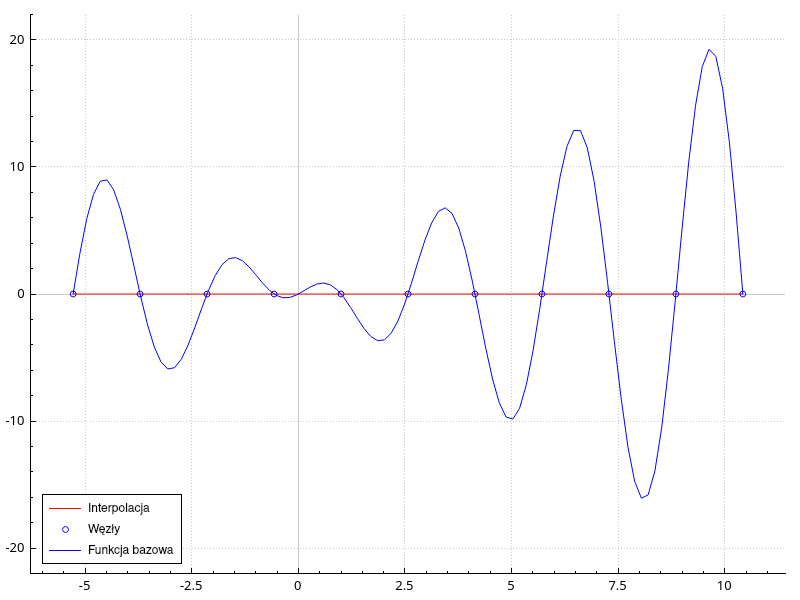
\includegraphics[width=0.8\textwidth]{img/n11Lagrange.png}
    \caption{Interpolacja Lagrange'a dla $n=11$}
    \label{fig:lagrange_n_11}
\end{figure}

\begin{figure}
    \centering
    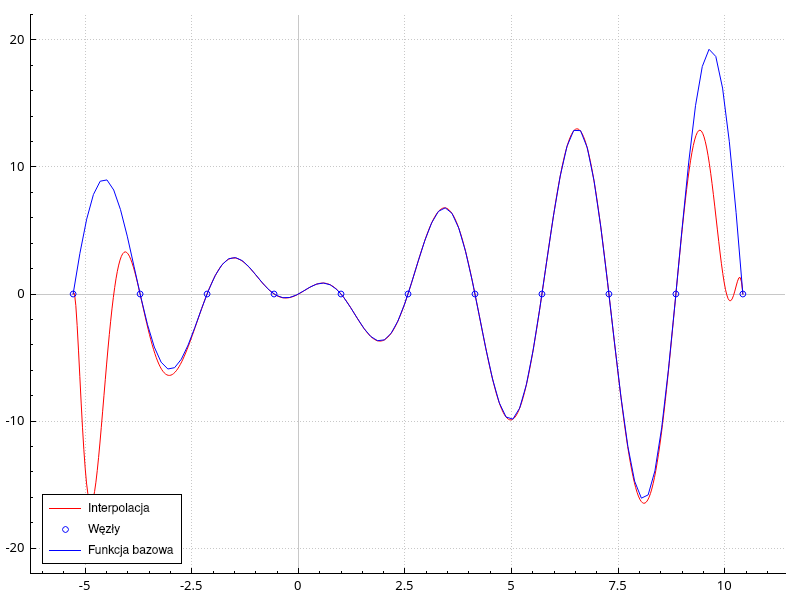
\includegraphics[width=0.8\textwidth]{img/n11Hermite.png}
    \caption{Interpolacja Hermite'a dla $n=11$}
    \label{fig:hermite_n_11}
\end{figure}

\begin{figure}
    \centering
    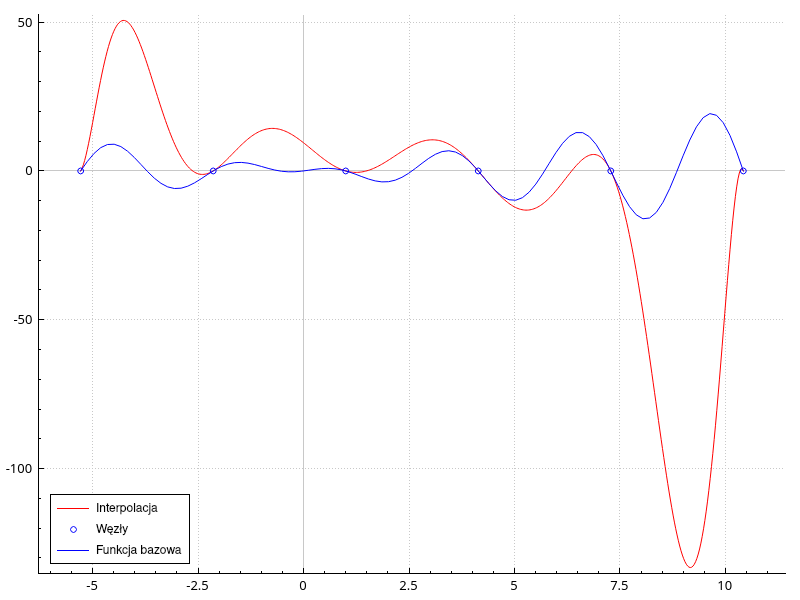
\includegraphics[width=0.8\textwidth]{img/n6Hermite.png}
    \caption{Interpolacja Hermite'a dla $n=6$}
    \label{fig:hermite_n_6}
\end{figure}

\subsection{Stabilność numeryczna}
\begin{table}[htbp]
\centering

\caption{Porównanie błędu maksymalnego Lagrange'a i Hermite'a dla dużej liczby węzłów.}
Jak moża zaobserwować w tabeli \ref{}
\label{tab:high_n_comparison}
\begin{tabular}{@{}ccccc@{}}
\toprule
\textbf{n} & \textbf{Lagrange (Równ.)} & \textbf{Hermite (Równ.)} & \textbf{Lagrange (Czeb.)} & \textbf{Hermite (Czeb.)} \\ \midrule
40 & 5.75e-06 & 1.85e+03 & 1.35e-11 & 3.05e+05 \\
50 & 1.63e-03 & 3.12e+12 & 2.84e-14 & 5.25e+15 \\
60 & 1.96e+00 & 9.90e+21 & 3.20e-14 & 7.00e+25 \\
70 & 1.36e+03 & 6.27e+31 & 2.58e-14 & 2.91e+35 \\
80 & 7.69e+05 & 8.97e+40 & 4.62e-14 & 1.35e+46 \\
90 & 7.34e+08 & 1.03e+50 & 5.33e-14 & 7.73e+55 \\ \bottomrule
\end{tabular}
\end{table}

\section{Wnioski}
\end{document}